\section{Implementation}

\subsection{Design Considerations for a Composability Manager}

The larger the HPC system, the greater the potential impact of dynamic composability of disaggregated components to energy efficiency and computational stability.  However, a centralized composabilty management layer must be scalable to be able to handle massive amounts of hardware telemetry, device states, device capabilities, and subscription information from large numbers of resources.  The OFMF is a centralized abstract management layer that exposes a RESTful API <cite> and incorporates DMTF Redfish <cite> and SNIA Swordfish <cite> schemas to enable infrastructure clients (e.g., users, management software, programming frameworks) to manage composition of, and fabric configuration to computational resources.  The OFMF transactions are stateless and lightweight, consisting of JSON data carried on Open Data Format (OData).  The Component Management Agents and the Composability Layer interact with the OFMF layer.  Through the use of Kafka \cite{kafka} or RabbitMQ \cite{rabbitmq} interfaces, the OFMF is designed to be able to scale.

Figure \ref{fig:ofmf} shows a higher level architectural diagram of the components making up the OFMF and a composability solution.  The left side of the diagram shows the user, admininisration, orchestration, automation, etc. Clients can be various Workload Managers, application and run-time libraries, monitoring systems, and System Administrators.  Clients interact with the Composability Layer between clients and the OFMF. The Composability Layer manages hardware resources to best provide run-time computational performance, energy efficiency, and resource monitoring by applying policies and updating subscribed clients with events. The Composability Layer allows clients to track the current state and coordinate resources that are within a disaggregated HPC system.

\begin{figure}[ComposableSolution]
  \centerline{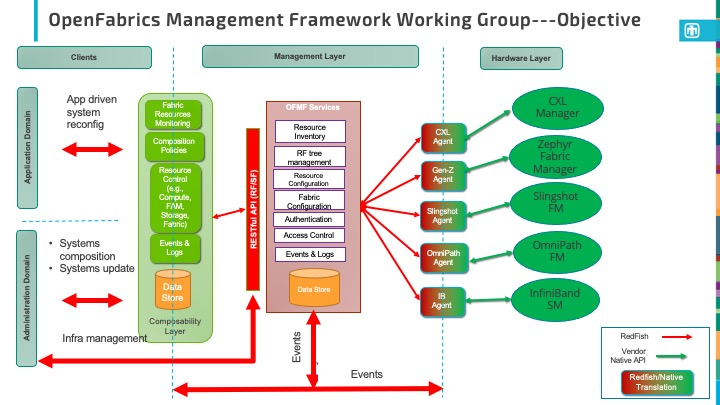
\includegraphics[width=\columnwidth]{ComposabilityHL_Diagram.jpeg}}
  \caption{Composability Solution based upon the OpenFabrics Management Framework}
  \label{fig:ofmf}
\end{figure}

The middle section of the diagram is a representation of the functional blocks making up the OFMF.  In the OFMF, an HPC's disaggregated infrastructure is represented under a single Redfish tree that includes all the fabrics and computational resources available. The OFMF services are subscription-based and represent a central repository for telemetry information, provisioning, and event logs.  Client requests received to the OFMF through the Composability Layer are forwarded to the appropriate fabric manager via dedicated light-weight technology-specific Agents. 

The Agents on the right translate between the OFMF and network fabric-specific providers.  These Agents provide access to network fabrics and trigger them to make the actual changes to their resources in their own technology-specific manner with their own technology-specific configuration tools.  

\subsection{Dynamic Composability In Action}



